\chapter{Mathematical Formulation}
\label{ch:formulation}

This chapter is the mathematical core of the project. It defines the decision problem the
honeypot faces (Sections~\ref{sec:mdp}--\ref{sec:reward}) and the learning algorithm with its
convergence conditions (Section~\ref{sec:learning}). It then defines the attacker model
(Section~\ref{sec:attackers}) and develops the exact evaluation method used in
Chapter~\ref{ch:results} (Sections~\ref{sec:exact}--\ref{sec:fit}).

\section{The Decision Problem}
\label{sec:mdp}

One SSH session is one \emph{episode}. The attacker issues commands $c_1, c_2, \dots, c_T$, and
before answering each one the honeypot (the \emph{agent}) chooses a response strategy. The
episode ends when the attacker disconnects, when the honeypot blocks, or at a limit.

\begin{definition}[Honeypot MDP]
The honeypot's problem is modelled as a finite MDP
$\mathcal{M} = (\mathcal{S}, \mathcal{A}, P, R, \gamma)$ with a terminal state $s_\bot$, where
\begin{itemize}
  \item $\mathcal{S} = \mathcal{K} \times \Phi$ is the set of observed states (Section~\ref{sec:state});
  \item $\mathcal{A} = \{\act{allow}, \act{delay}, \act{fake}, \act{tarpit}, \act{block}\}$;
  \item $P(s' \mid s, a)$ is induced by the attacker's behaviour and is unknown to the agent;
  \item $R(s, a, s')$ is the reward of Section~\ref{sec:reward}; and
  \item $\gamma = 0.9$ is the discount factor.
\end{itemize}
\end{definition}

\section{State Space}
\label{sec:state}

\paragraph{Command category.} A deterministic, rule-based classifier maps each command line to
one of ten categories $\kappa \in \mathcal{K}$. Each category has an \emph{intelligence value}
$v(\kappa)$: how much an analyst learns from seeing it (Table~\ref{tab:categories}). A chained
line (\code{cd /tmp \&\& wget \dots \&\& chmod +x \dots}) takes the highest-value category among
its parts, since that is the intent the attacker revealed.

\begin{table}[H]
\centering
\small
\begin{tabularx}{\textwidth}{@{}l>{\raggedright\arraybackslash}Xc@{}}
\toprule
\textbf{Category} $\kappa$ & \textbf{Examples} & $v(\kappa)$ \\
\midrule
recon & \code{uname -a}, \code{id}, \code{ps aux}, \code{cat /proc/cpuinfo} & 1 \\
fs\_browse & \code{ls}, \code{cd}, \code{find}, \code{cat} (non-sensitive) & 1 \\
cred\_access & \code{cat /etc/shadow}, \code{cat \textasciitilde/.ssh/id\_rsa}, \code{cat .env} & 3 \\
download & \code{wget}, \code{curl}, \code{tftp}, \code{git clone} & 4 \\
execute & \code{chmod +x}, \code{./payload}, \code{sh script.sh} & 4 \\
persist & \code{crontab -}, \code{>> authorized\_keys}, \code{useradd} & 5 \\
privesc & \code{sudo -i}, \code{su}, \code{passwd} & 3 \\
cleanup & \code{history -c}, \code{rm /var/log/*}, \code{unset HISTFILE} & 4 \\
benign & \code{echo}, \code{clear}, \code{exit} & 0 \\
unknown & anything unmatched & 1 \\
\bottomrule
\end{tabularx}
\caption{Command categories and their intelligence values.}
\label{tab:categories}
\end{table}

\paragraph{Session phase.} The phase summarises how far the session has progressed:
\[
\phi_t = \begin{cases} \text{early} & t \le 3,\\ \text{mid} & 4 \le t \le 10,\\ \text{late} & t \ge 11. \end{cases}
\]
The state is $s_t = (\kappa_t, \phi_t)$, so $|\mathcal{S}| = 30$ and the Q-table has 150 entries.
This is deliberately small: it can be learned from thousands of sessions rather than millions,
and every entry can be shown on the dashboard.

\paragraph{Partial observability.} The process is \emph{not} Markov in $s_t$. What an attacker
does next depends on who they are (a scripted bot, an unskilled human, a skilled operator),
and the honeypot cannot observe that. Section~\ref{sec:posterior} shows that the phase is
nevertheless informative about the hidden type, which is why it belongs in the state.

\section{Actions}

\begin{table}[H]
\centering
\small
\begin{tabularx}{\textwidth}{@{}lXc@{}}
\toprule
\textbf{Action} & \textbf{Behaviour} & $\chi(a)$ (s) \\
\midrule
\act{allow} & Return the faithful emulated output. & 0 \\
\act{delay} & Wait $U(1,4)$ s, then return faithful output. & 2.5 \\
\act{fake} & Plant decoy files (credential files, \code{.env}, \code{.my.cnf}, \code{wp-config.php}) and add decoy entries to \code{ps} and \code{env} output. & 0 \\
\act{tarpit} & Wait 4--7 s, then dribble the output a few bytes at a time ($\approx$10--15 s in total). & 15 \\
\act{block} & Close the connection (terminal). & 0 \\
\bottomrule
\end{tabularx}
\caption{Response actions and their expected friction cost $\chi(a)$.}
\label{tab:actions}
\end{table}

\section{Reward}
\label{sec:reward}

The reward measures the intelligence gained by letting the session continue, net of the friction
imposed:
\begin{equation}
r_t = \mathbb{1}[\text{cont}_t]\,\big(w_e + w_v\, v(\kappa_{t+1})\big)
      \;-\; w_c\,\chi(a_t)
      \;+\; w_b\,\mathbb{1}\big[a_t = \act{block},\ \kappa_t = \text{cleanup},\ \phi_t = \text{late}\big],
\label{eq:reward}
\end{equation}
with defaults $w_e = 1$, $w_v = 0.5$, $w_c = 0.02$ and $w_b = 2$. Each further command is worth
$w_e$, and high-value next commands are worth more. Friction is mildly penalised. \act{block}
is normally bad because it ends the flow of information, but it earns a bonus once a late
session is covering its tracks. The \emph{attrition} variant used in Chapter~\ref{ch:results}
sets $w_c = -0.05$, so that wasting attacker time is rewarded.

The agent maximises the expected discounted return $\E\big[\sum_{t} \gamma^{t-1} r_t\big]$.
Because the return is defined by a modelling choice (the weights), the evaluation also reports
reward-independent quantities: expected commands per session and expected intelligence
per session.

\section{Learning Algorithm}
\label{sec:learning}

\paragraph{Q-learning.} After observing $(s_t, a_t, r_t, s_{t+1})$, the agent updates
\begin{equation}
Q(s_t,a_t) \leftarrow Q(s_t,a_t) + \alpha_n(s_t,a_t)\Big[r_t + \gamma \max_{a'} Q(s_{t+1},a') - Q(s_t,a_t)\Big],
\label{eq:q}
\end{equation}
with $Q(s_\bot,\cdot) = 0$. SARSA replaces $\max_{a'} Q(s_{t+1}, a')$ by $Q(s_{t+1}, a_{t+1})$.
The behaviour policy is $\varepsilon$-greedy with $\varepsilon_k = \max(0.05,\ 0.3 \times
0.995^k)$ after $k$ episodes. Initially $Q(s,\act{allow}) = 0.5$ and every other entry is $0$,
so an untrained honeypot behaves like a conventional one.

\paragraph{Step size.} Let $n = n(s,a)$ be the number of times the pair has been updated. We use
\begin{equation}
\alpha_n = n^{-\omega}, \qquad \omega = 0.7 .
\label{eq:alpha}
\end{equation}

\begin{proposition}[Convergence, Watkins and Dayan~\cite{watkins1992q}]
In a finite MDP with bounded rewards, if every state--action pair is updated infinitely often
and
\[
\textstyle\sum_{n} \alpha_n = \infty, \qquad \sum_{n} \alpha_n^2 < \infty,
\]
then the Q-learning iterates converge to $Q^*$ with probability one.
\end{proposition}

For $\alpha_n = n^{-\omega}$ both sums behave like $p$-series: $\sum n^{-\omega}$ diverges
for $\omega \le 1$ and $\sum n^{-2\omega}$ converges for $\omega > \tfrac12$. The conditions
therefore hold exactly when $\tfrac12 < \omega \le 1$. A \emph{constant} step size violates the
second condition. Its estimate keeps fluctuating: for a quantity estimated from i.i.d.\ targets
with variance $\sigma^2$, the stationary variance of the exponentially weighted average is
\[
\operatorname{Var}\big[Q_\infty\big] = \sigma^2 \sum_{j\ge 0} \alpha^2 (1-\alpha)^{2j}
= \sigma^2 \frac{\alpha}{2-\alpha},
\]
so with $\alpha = 0.1$ the estimate keeps a standard deviation of about $0.23\,\sigma$ forever.
Chapter~\ref{ch:results} shows that this noise floor is larger than the true differences
between actions in the most frequently visited states, so the greedy policy is decided by
noise. The first update of \eqref{eq:alpha} has $\alpha_1 = 1$, which also replaces the
arbitrary initial value with a real sample.

Two caveats apply. (i) The proposition assumes an MDP, but the honeypot faces a POMDP. Q-learning
on observations need not converge to the best memoryless policy~\cite{singh1994pomdp}, so we
\emph{measure} the gap instead of assuming it is zero. (ii) A convergent schedule stops adapting,
while a real attacker population drifts. For long deployments a floor $\alpha_n \ge \alpha_{\min}$
trades a small, bounded noise level for tracking.

\section{Attacker Population Model}
\label{sec:attackers}

To evaluate policies we need an environment whose dynamics are known to the \emph{evaluator}
(though never to the agent). An attacker of type $k$ is a Markov chain over categories with an
action-dependent continuation probability:
\begin{align}
\Pr(\kappa_1 = c \mid k) &= \mu_k(c), \\
\Pr(\text{continue} \mid k, \kappa_t = c, a_t = a) &= q_k(c,a) = \min\!\big(0.98,\ (1-e_k(c))\, m_k(c,a)\big), \\
\Pr(\kappa_{t+1} = c' \mid k, c, a, \text{continue}) &= N_k(c,a,c'),
\end{align}
where $e_k(c)$ is the attacker's own exit probability, and $m_k(c,a)$ is a reaction multiplier
($m_k(c,\act{block}) = 0$). For most actions $N_k(c,a,\cdot)$ is the attacker's base transition
row. After \act{fake} on credential access it is mixed 50/50 with a ``chase the honeytoken''
distribution. The population is a mixture with weights $w_k$ over three types:

\begin{table}[H]
\centering
\small
\begin{tabularx}{\textwidth}{@{}lcX@{}}
\toprule
\textbf{Type} & \textbf{Weight} & \textbf{Behaviour and reactions} \\
\midrule
bot & 0.60 & Scripted recon $\rightarrow$ download $\rightarrow$ execute; exits quickly. Indifferent to content; \act{delay} $\times 0.90$, \act{tarpit} $\times 0.35$ (time-outs). \\
script kiddie & 0.25 & Browses and hunts for credentials; impatient. \act{delay} $\times 0.80$, \act{tarpit} $\times 0.30$; \act{fake} on cred\_access $\times 1.15$ and steers towards credentials and downloads. \\
operator & 0.15 & Patient and methodical. \act{tarpit} $\times 0.60$; \act{fake} on cred\_access $\times 1.20$ (chases the decoy) and steers towards download, persistence and privilege escalation; \act{fake} on recon or browsing $\times 0.85$ (fabricated system data is inconsistent). \\
\bottomrule
\end{tabularx}
\caption{Attacker types in the balanced population. The bot-heavy mix uses weights (0.85, 0.10, 0.05) and the human-heavy mix (0.30, 0.35, 0.35).}
\label{tab:types}
\end{table}

These parameters are modelling assumptions informed by qualitative findings about SSH attackers,
not measurements. Section~\ref{sec:fit} shows how to estimate them from data, and
Chapter~\ref{ch:results} tests how sensitive the conclusions are to them.

\section{Exact Policy Evaluation}
\label{sec:exact}

Because the model is known, the expected performance of any policy can be \emph{computed}
rather than estimated by simulation.

\paragraph{Augmented chain.} Let $x = (k, c, t)$ with $t$ capped at $T = 11$; from $t = 11$
on, the phase is always late. Then $|X| = 3 \times 10 \times 11 = 330$. Under action $a$:
\[
P_a\big((k,c,t), (k,c',\min(t+1,T))\big) = q_k(c,a)\, N_k(c,a,c'),
\]
and with probability $1 - q_k(c,a)$ the process is absorbed. The expected immediate reward
is \eqref{eq:reward} in expectation:
\[
r_a(k,c,t) = q_k(c,a) \sum_{c'} N_k(c,a,c') \big(w_e + w_v v(c')\big) - w_c \chi(a)
+ w_b\,\mathbb{1}[a = \act{block}, c = \text{cleanup}, t = T].
\]

\paragraph{Policies over observations.} A (possibly stochastic) honeypot policy $\pi(a \mid c,
\phi)$ sees only the category and the phase. It induces
$P_\pi(x, \cdot) = \sum_a \pi(a \mid c, \phi(t))\, P_a(x, \cdot)$ and similarly $r_\pi$.
Every row of $P_\pi$ sums to at most $0.98$, so $P_\pi$ is strictly sub-stochastic and
$I - \gamma P_\pi$ and $I - P_\pi$ are invertible.

\begin{proposition}[Exact metrics]
Let $\mu_0(k,c,1) = w_k \mu_k(c)$ be the start distribution, and define
\[
V_\pi = (I - \gamma P_\pi)^{-1} r_\pi, \qquad N_\pi = (I - P_\pi)^{-1}.
\]
Then the expected discounted return is $\mu_0^\top V_\pi$, the expected number of commands per
session is $\mu_0^\top N_\pi \mathbf{1}$, and the expected intelligence per session is
$\mu_0^\top N_\pi\, v$, where $v(x) = v(c)$.
\end{proposition}
\noindent The first identity is the Bellman equation for a fixed policy~\cite{puterman1994mdp}.
The second is the fundamental matrix of an absorbing chain: $(N_\pi)_{xy}$ is the expected
number of visits to $y$ starting from $x$~\cite{kemeny1960finite}. Each evaluation is a
$330 \times 330$ linear solve, which takes about 3\,ms.

\paragraph{Benchmarks.}
\begin{itemize}
  \item \textbf{Oracle.} If the honeypot could observe $x$ (in particular the type $k$), the
    optimal value would satisfy $V^*(x) = \max_a \big[r_a(x) + \gamma P_a(x,\cdot) V^*\big]$.
    Value iteration solves this. No honeypot policy can exceed it.
  \item \textbf{Best observable policy.} The best deterministic policy over $(c, \phi)$ maximises
    $\mu_0^\top V_\pi$ over $5^{30}$ candidates. Optimising memoryless POMDP policies is NP-hard
    in general, so we use coordinate ascent with exact evaluation inside: change one observable
    state's action at a time, keep strict improvements, and use eight restarts. All restarts reach
    the same policy. The result is the realistic ceiling for an agent with the honeypot's state
    representation.
\end{itemize}

\section{Type Posterior and the Role of Phase}
\label{sec:posterior}

Under a policy $\pi$, the probability that a session reaching command $t$ belongs to type $k$
follows from propagating $\mu_0$ through $P_\pi$ one step at a time and normalising the mass
at index $t$ by type. Figure~\ref{fig:posterior} shows the result under the static policy.
Bots are 60\% of sessions at $t=1$ but only 16\% of sessions that reach $t \ge 11$, while
operators rise from 15\% to 54\%. The phase is therefore a cheap proxy for the hidden type.

\begin{figure}[H]
\centering
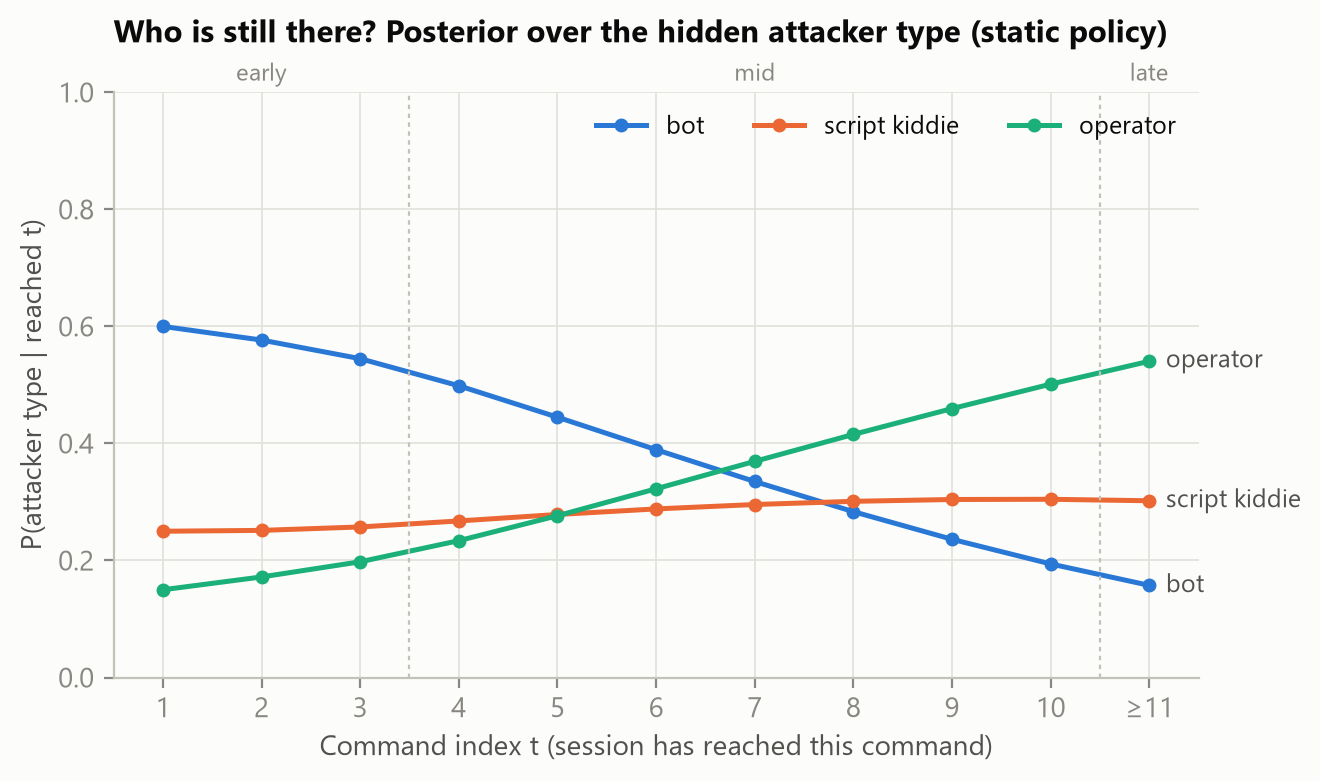
\includegraphics[width=0.85\textwidth]{fig_type_posterior.png}
\caption{Posterior probability of each attacker type given that the session has reached
command $t$ (static policy, balanced population).}
\label{fig:posterior}
\end{figure}

\section{Estimating the Model from Data}
\label{sec:fit}

Given the category sequences of captured sessions, the likelihood of a chain with initial
distribution $\mu$, transition matrix $P$ and exit probabilities $e$ is
\[
L = \prod_{\text{sessions}} \mu(c_1) \prod_{i=1}^{n-1} \big(1-e(c_i)\big) P(c_i, c_{i+1}) \cdot e(c_n).
\]
The likelihood factorises over $\mu$, over each row of $P$, and over each $e(c)$, and each factor
is a multinomial or Bernoulli likelihood. The maximiser is therefore the normalised counts:
\[
\hat\mu(c) = \frac{\#\text{starts at } c}{\#\text{sessions}}, \quad
\hat P(c,c') = \frac{\#(c \to c')}{\#(c \to \cdot)}, \quad
\hat e(c) = \frac{\#\text{ends at } c}{\#\text{visits to } c}.
\]
Laplace smoothing adds a pseudo-count to each transition. Fitted to sessions served by the
static policy, these estimates describe the attackers' own behaviour. Reaction multipliers can
be estimated only from sessions in which different actions were taken, which the live learner's
exploration provides.
